\documentclass{sig-alternate-05-2015}
%\usepackage[margin=.7in]{geometry} 
\usepackage{amsmath,amssymb}
\usepackage{mathpartir}
\usepackage{scrextend}
\usepackage{hyperref}


\begin{document}
\setcopyright{none}

\title{Human Action Recognition Using Scene Context}
\numberofauthors{1}
\author{
  \alignauthor Qiuwei Shou\\
  \affaddr{Indiana University}\\
  \email{qiuwshou@umail.iu.edu}
}
\makeatletter
\def\@copyrightspace{\relax}
\makeatother

\maketitle

\section{Introduction}
Human action recognition has been studied widely in computer vision.Many researches have been done on static camera and surveillance to recognize action in past decades.
Recently more and more approaches have been studied to capture actions in dynamic videos. It becomes a more challenging and interesting task to detect or recognize action in highly unconstrained dataset.
Many state-of-the-art methods developed by deep learning approaches have shown good performance on web datasets like UCF50 and  HMDB51. 
Image based model also have been improved by taking account the scene information.\par
There are various approaches to combine the scene information like using CRF and super pixels. In this project, we will try to develop a image based model by applying CSIFT\cite{vandeSandeTPAMI2010} to capture scene context.
The project is inspired by \cite{Reddy:2013:RHA:2508580.2508584}. We use a similar architecture and different setup which will be describe in section \ref{sec:eval}. 
The reference implementations are color sift \cite{vandeSandeTPAMI2010} and opencv\cite{opencv}.
In section \ref{sec:prob}, we will briefly describe the problem and scene context descriptor,
in section \ref{sec:method} we will describe our implementation of applying CSIFT and motion descriptors,
in section \ref{sec:eval} we will evaluate our method using UCF50 dataset\cite{ucf50}
and we conclude this project in section \ref{sec:con}.

\section{Scene Descriptors}\label{sec:prob}
Scene context is useful to put constrain on the actions.  For example, skiing and skate boarding have similar motion patterns, but these actions take place in different context and scene. Skiing happens
on snow, which is very different from where skate boarding is done\cite{Reddy:2013:RHA:2508580.2508584}. Many actions are associated with particular scene and context. 
Many researches have discovered the dependency of particular actions upon certain scene using probabilistic model \cite{Hoiem2008}. It have been shown that combing scene context can increase the accuracy of classification. 
We define the scene context as stationary pixels in a image. We compute the dense optical flow $(u,v)$ at each pixel by using Gunner Farneback's algorithm\cite{Farneback:2003:TME:1763974.1764031}. 
We use CSIFT\cite{vandeSandeTPAMI2010} to distinguish the scene context. For example, skiing usually happens in the snow environment which will generate distinct CSIFT descriptor.

\section{Proposed Approach}\label{sec:method}
\begin{figure}[h]
 \centering
  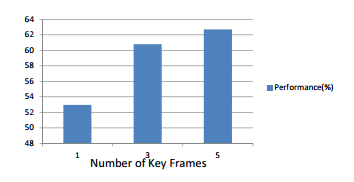
\includegraphics[scale=0.8]{fig/key_frame.png}
  \caption{Performance vs Number of key frames}
  \label{fig:frames}
  \cite{Reddy:2013:RHA:2508580.2508584}
\end{figure}
We define the scene context as stationary pixels in a image. For each video clip, we sample 4 key frames evenly through the whole video. Using more key frames will increase the accuracy with increasing the run time (see figure \ref{fig:frames}). 
We compute the dense optical flow $(u,v)$ at each pixel between two consecutive frame, using Gunner Farneback's algorithm\cite{Farneback:2003:TME:1763974.1764031}. Apply in a threshold to the displacement, we decide if a pixel is moving or stationary. We compute the CSIFT for the whole image then separate pixels into stationary group $SP$ and moving group $MP$ by pixel index. We extract CSIFT from both group and use BOW paradigm to create two histogram representations of 200 codebook (see figure \ref{fig:flow}). 
We also concatenate all the dense optical flows for consecutive key frames and create a histogram representation $M$ with the same number of codebook for each video clip. We first train the scene context descriptor and motion descriptor separately by SVM classifier\cite{Chang:2011:LLS:1961189.1961199}. Then we use early fusion to combine the two feature descriptors together. See figure \ref{fig:flow} for the work flow. \par 
\begin{figure}[h]
 \centering
  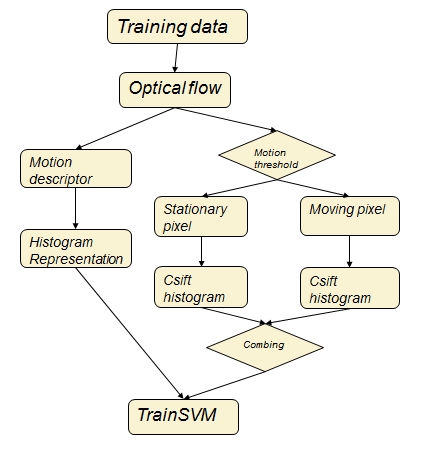
\includegraphics[scale=0.6]{fig/flow.png}
  \caption{Proposed Approach}
  \label{fig:flow}
\end{figure}

\section{Evaluation}\label{sec:eval}
\begin{figure}[h]
\centering
  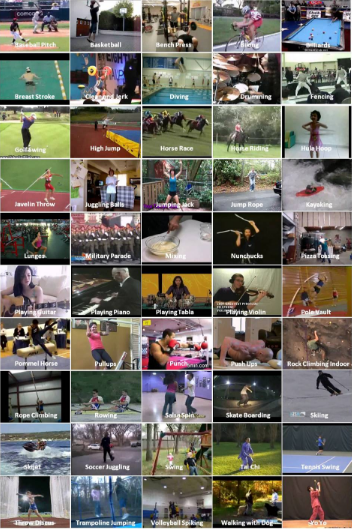
\includegraphics[scale=0.5]{fig/ucf50.png}
  \caption{A snapshot of UCF50 dataset}
  \label{fig:ucf50}
\end{figure}
In this section we will conducting evaluation of our method using UCF50 dataset \cite{ucf50}.
UCF50 is a collection of web videos with 50 categories, and  we will use our method to classify the category of videos. Under each category there are 25 groups of video. The video clips in the same  group are taken from the same video. 
We split data into training set and test set half by half evenly through the group to guarantee we have the training data and test data from the same video. by key frames of 4 we totally sampled 26724 images of 240*320 dimensions. For each one we extact 1957 CSIFT descriptors of 384 dimensions vector by dense sampling at every 6 pixels.
We use 2 for threshold to distinguish the moving pixel and stationary pixel. Averagely using the motion descriptor we achieve about $48\%$ accuracy  for only using motion descriptor and $45\%$ by only using scene context descriptor. Combing two descriptors achieve overall performance of $54\%$ . In the \cite{Reddy:2013:RHA:2508580.2508584} the performance for using motion descriptor and scene descriptor are $53\%$ and $49\%$, and late fusion of both gives overall performance of $68\%$ with 1000 dimension codebook and 3 key frames. So we didn't achieve large improvements by early fusion. Because the original experiment details aren't fully explained in the \cite{Reddy:2013:RHA:2508580.2508584} and there are many parameters need to be tuned. There more details could be explored to increase the performance. According to the results in the figure \ref{fig:other_result}, it shows that the experiment setup can affected the performance. Also the threshold value might be critical. If it is too small we might lose context information for the object and action, or if it is too larger we can lost scene context information. The window stride and pyramid scale can affect the performance of dense optical flow. Increase key frames and dimension of codebook definitely increase the performance. Also the assumption is not flawless because we assume that the scene is homogeneous. For the actions that could happen in different scenes it might lose the accuracy. Moreover, the length of video clip is various. It causes the ambiguity to produce the same motion patterns for the video clip if the frames are sampled at differ fps rate. Splitting the data half by half might give us less training data so the classifier is not learned well. Also we use 10 iteration and 0.1 epsilon for generating codebook, which might not be converged. 
\begin{figure}[h]
 \centering
  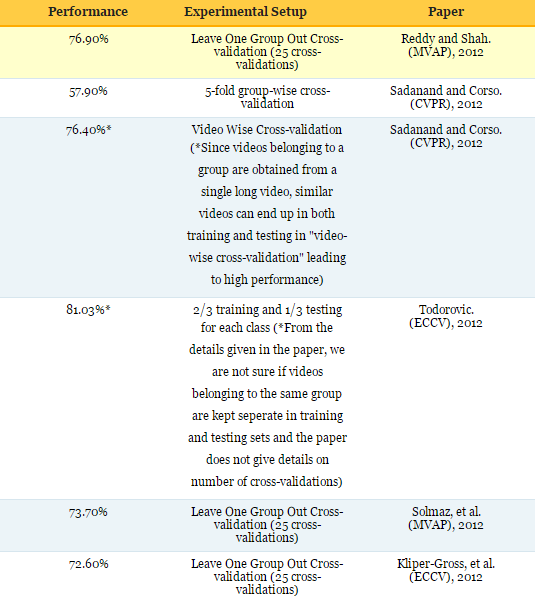
\includegraphics[scale=0.5]{fig/other_result.png}
  \caption{Other results on the UCF50 dataset}
  \label{fig:other_result}
\end{figure}

\section{Conclusion}\label{sec:con}
We didn't achieve the good performance with higher key frames than the \cite{Reddy:2013:RHA:2508580.2508584}. But we have proved that combing scene context definitely help to increase the accuracy of the classification by $6\%$. Using image based model doesn't require large amount data set and can work for unconstrained data well. But it can hit the boundary easily. As the deep learning is the big trend in the computer vision, for the future enhancement, we want to apply CNN for scene classification with more appropriate descriptors. 



\bibliographystyle{abbrv}
\bibliography{bib/refs}

\clearpage


\end{document}
